\subsection{Testläufe}
Im folgenden werden die verschiedenen Testläufe genau beschrieben. Für alle Testläufe gilt, dass das AUV zuerst 30 Meter geradeaus fährt, bevor es auf das Objekt trifft, damit eine stabile Fahrt erreicht wird und die Schwankungen beim anfänglichen Beschleunigen die Ergebnisse nicht verfälschen. Ebenso wird auch gewährleistet, dass das AUV stets direkt auf das Objekt trifft, da dass Explorieren und Auffinden des Objektes nicht Teil der Arbeit ist.\\
Zu jedem Testlauf befindet sich auf der CD ein Video, in dem das AUV von oben, die Rohbilder der Kamera, die Ausgabe der Objekterkennung und das berechnetet Polynom zu sehen ist.
\subsubsection{Gerader Verlauf}
Für die ersten Tests wurde ein 100 Meter langes Objekt gerade in die Simulationsumgebung eingefügt. Dieses Objekt ist in mehreren Bereichen vom Meeresboden leicht bis komplett bedeckt. 

\begin{figure}[H]
\begin{tabular}{cc}
\multicolumn{2}{c}{\subfloat[Fahrtverlauf des AUVs (rot) an einem geraden Objekt (blau). Nach erstem Sichtkontakt zum Objekt ist ein einpendeln auf die gerade Linie zu beobachten.]{\includegraphics[height=0.4\textheight,width=\textwidth]{/testlaeufe/gradeGut/auvroute.jpg}}}\\
\subfloat[Fehler der AUV Position zur echten Position des Objektes. Auch hier ist zu beobachten, dass ein großer Fehler zu Beginn des Objektes auftritt, der beim Fahrtverlauf weiter verringert wird.]{\includegraphics[height=0.3\textheight,width=0.5\textwidth]{/testlaeufe/gradeGut/groundTruthPosition.jpg}}&
\subfloat[Fehler der detektierten Objektposition zur echten Objektposition. In Betrachtung von \textit{b)} ist zu beobachten, dass der Fehler der detektierten Objektposition größer ist, als der Fehler im daraus resultierenden Fahrtverlauf.]{\includegraphics[height=0.3\textheight,width=0.5\textwidth]{/testlaeufe/gradeGut/groundTruth.jpg}}
\end{tabular}
\caption{Testlauf an einem geraden Objekt. Nach anfänglich größeren Fehler folgt das AUV dem Objekt mit nur sehr geringem Fehler. Das Einpendeln ist auf die Berechnug des Polynoms zurückzuführen, da bei wenigen Punkten zu Beginn der Verlauf noch nicht eindeutig als Gerade bestimmbar ist. Siehe hierfür Kapitel \ref{sec_pendel}}
\end{figure}

\subsubsection{Kurve}
Nach den Tests zum geraden Verlauf wurden kurvige Objekte mithilfe von Polynomial- und Exponentialfunktionen in die Simulation eingefügt. Hierbei wurde darauf geachtet kein Polynom zweiten Grades zu verwenden, um dem Regressionsverfahren keine perfekte Lösung zu bieten.\\
Ziel dieser Tests ist es zu zeigen, dass das Folgen einer Links- sowie Rechtskurve und auch ein wechseln zwischen beiden Kurvenarten möglich sind. Für letzteres wurde eine Sinuskurve genutzt, um ein entsprechendes Objekt zu erzeugen.


\begin{figure}[H]
\begin{tabular}{cc}
\multicolumn{2}{c}{\subfloat[]{\includegraphics[height=0.4\textheight,width=\textwidth]{/testlaeufe/linkskurve/auvroute.jpg}}}\\
\subfloat[]{\includegraphics[height=0.3\textheight,width=0.5\textwidth]{/testlaeufe/linkskurve/groundTruthPosition.jpg}}&
\subfloat[]{\includegraphics[height=0.3\textheight,width=0.5\textwidth]{/testlaeufe/linkskurve/groundTruth.jpg}}
\end{tabular}
\end{figure}

\begin{figure}[H]
\begin{tabular}{cc}
\multicolumn{2}{c}{\subfloat[]{\includegraphics[height=0.4\textheight,width=\textwidth]{/testlaeufe/rechtskurve/auvroute.jpg}}}\\
\subfloat[]{\includegraphics[height=0.3\textheight,width=0.5\textwidth]{/testlaeufe/rechtskurve/groundTruthPosition.jpg}}&
\subfloat[]{\includegraphics[height=0.3\textheight,width=0.5\textwidth]{/testlaeufe/rechtskurve/groundTruth.jpg}}
\end{tabular}
\end{figure}

\begin{figure}[H]
\begin{tabular}{cc}
\multicolumn{2}{c}{\subfloat[]{\includegraphics[height=0.4\textheight,width=\textwidth]{/testlaeufe/sinusGut/auvroute.jpg}}}\\
\subfloat[]{\includegraphics[height=0.3\textheight,width=0.5\textwidth]{/testlaeufe/sinusGut/groundTruthPosition.jpg}}&
\subfloat[]{\includegraphics[height=0.3\textheight,width=0.5\textwidth]{/testlaeufe/sinusGut/groundTruth.jpg}}
\end{tabular}
\end{figure}

\begin{figure}[H]
\begin{tabular}{cc}
\multicolumn{2}{c}{\subfloat[]{\includegraphics[height=0.4\textheight,width=\textwidth]{/testlaeufe/S-Kurve_Gut/auvroute.jpg}}}\\
\subfloat[]{\includegraphics[height=0.3\textheight,width=0.5\textwidth]{/testlaeufe/S-Kurve_Gut/groundTruthPosition.jpg}}&
\subfloat[]{\includegraphics[height=0.3\textheight,width=0.5\textwidth]{/testlaeufe/S-Kurve_Gut/groundTruth.jpg}}
\end{tabular}
\end{figure}

Außerdem wurde noch eine Kurve nach einer langen Geraden erzeugt. Hiermit wird getestet, ob auch wechselnden geometrischen Strukturen gefolgt werden kann.

\subsection{Kreisbahn}
Für die finalen Tests wurden Kreisbahnen in Form von Ellipsen verwendet. Eine Ellipse erfüllt einige Eigenschaften, die für die Arbeit nicht trivial zu lösen sind. Zum einen gibt es verschieden stark gebogene Kurven und fast gerade Abschnitte. Zum anderen gibt es ständig Abschnitte, die parallel zur $Y-Achse$ verlaufen.\\

\begin{figure}[H]
\begin{tabular}{cc}
\multicolumn{2}{c}{\subfloat[]{\includegraphics[height=0.4\textheight,width=\textwidth]{/testlaeufe/kreiszweimalrum-gut/auvroute.jpg}}}\\
\subfloat[]{\includegraphics[height=0.3\textheight,width=0.5\textwidth]{/testlaeufe/kreiszweimalrum-gut/groundTruthPosition.jpg}}&
\subfloat[]{\includegraphics[height=0.3\textheight,width=0.5\textwidth]{/testlaeufe/kreiszweimalrum-gut/groundTruth.jpg}}
\end{tabular}
\end{figure}